\documentclass[11pt,a4paper]{article}
\usepackage[utf8]{inputenc}
\usepackage[margin=2.5cm]{geometry}
\usepackage{amsmath,amssymb}
\usepackage{booktabs}
\usepackage{enumitem}
\usepackage{graphicx}
\usepackage[round,authoryear]{natbib}
\usepackage{microtype}
\usepackage[hidelinks]{hyperref}
\usepackage{url}

\title{A Bilinear Predictor Improves LeWorldModel Planning\\on Two-Rooms but Underperforms on PushT}
\author{Hassan Akaou\\
\small Independent researcher, France\\
\small \url{https://github.com/sahnas/stigmergic-module-routing}}
\date{October 2026}

\begin{document}
\maketitle

\begin{abstract}
We report a preregistered study that follows one idea from a synthetic compositional world to a released world model, and keeps its negative results. The idea: small learning modules coordinated by stigmergic traces (reinforced by use, evaporated when the task symbol is solicited), with the least committed module recruited when one fails. In eleven toy experiments, with the mechanism never tuned and opponents tuned on separate seeds, the mechanism gives resilience to module loss without a routing gradient, on par with sliding-window and discounted UCB; it does not beat routers trained by gradient, dense or sparse; per-module alarm thresholds bring nothing; and it discovers no compositional structure unless each module receives its own local error, in which case trace routing finds the shared structure with a cleaner decomposition than dense or sparse gradient routers. Five further experiments show that the mechanism protects no function by itself: once no spare capacity is left, a specialist is consumed under every recruitment rule, and only reserves held back until an event preserve it. On the frozen representation of the released LeWorldModel for Two-rooms, with a scenario of changing dynamics, banks of specialists with freezing and held-back reserves are not better than a reservoir replay buffer of 20,000 windows on any retention measure, which stops the line by the preregistered rule. On the way we found that LeWorldModel's own predictor, retrained from scratch on the frozen released encoder with a loss on the last position of three real frames, reaches eleven times lower latent error on that setting and plans far worse (36\% vs 85\% success on Two-rooms); six offline diagnostics, all starting from three real frames, failed to explain it, and an external reading of the recipe did: the planner starts from one frame, the official loss supervises every position, and the retrained network had an error of 1.18 at a context of one frame. Retrained with the official loss, it plans like the released predictor (84, 85, 89, 81 against 85, 83, 87, 80 on four evaluation seeds) with twelve times lower latent error. We then replaced the predictor by a ridge-fitted bilinear predictor, linear in the embedding and bilinear in embedding and action, with ten times higher held-out one-step latent error than the released predictor (0.69 vs 0.067). On Two-rooms, with the authors' evaluation unchanged, it increased planning success on three preregistered evaluation seeds (99, 100 and 96 of 100 against 83, 87 and 80), after an exploratory 97 against 85 on the authors' seed, and above the corrected neural predictor on every seed with every discordant episode but three in its favour. The tested ablations support a contribution from the bilinear state-action terms (57\% without them on one seed). On this evaluation, held-out latent error does not rank the three predictors by planning success; the mechanism behind the bilinear predictor's advantage, including its interaction with the planner's action constraints, remains unresolved. A nineteenth experiment applies the same fixed fitting recipe to the released PushT encoder. The bilinear predictor succeeds in 35, 40, 39 and 36 of 100 tasks, against 89, 86, 89 and 85 for the released predictor and 93, 94, 91 and 89 for the correctly retrained network. Both preregistered comparisons fail on every confirmatory seed, with a large disadvantage rather than a ceiling tie. The planning gain is therefore confined to Two-rooms among the two tested environments. Code, data, preregistrations, code hashes, seed ledgers and a provenance report are public.
\end{abstract}

\section{Introduction}

Modular neural systems need a way to decide which module handles which part of a task. The dominant answer is a router trained jointly with the modules by gradient descent, as in mixtures of experts \citep{jacobs1991experts,shazeer2017moe}. Another family routes with reinforcement learning \citep{rosenbaum2018routing}, and a third coordinates modules through a shared workspace \citep{goyal2022workspace}; see \citet{pfeiffer2023modular} for a survey. In some settings, however, the router cannot receive gradients: modules may be physically separated, heterogeneous, added or removed during operation, or simply not differentiable end to end. Such settings also raise a robustness question: what happens when a module fails?

Social insects solve a related problem without a central controller. Ants coordinate through traces deposited in the environment, a mechanism called stigmergy \citep{grasse1959}, which inspired ant colony optimisation \citep{dorigo1996antsystem} and ant-based network routing \citep{dicaro1998antnet}. Division of labour emerges from individual response thresholds \citep{bonabeau1996threshold,theraulaz1998reinforcement}, and recruitment of idle workers has been transferred to cooperative robots \citep{krieger2000robots}.

We ask whether these ingredients, transposed to routing between modules that learn during operation, produce a useful coordination mechanism, and where it breaks. The mechanism combines evaporating traces on symbol-to-module edges, an alarm on abnormal quality drops, and recruitment of the least committed module. We test it in a deliberately small synthetic world, using preregistered hypotheses \citep{nosek2018preregistration}, separate development and test seeds, tuned opponents and an untuned mechanism.

Our contributions are empirical and include negative results, reported at the same rank as the positive ones. (i) In its most defensible form, the mechanism is a distributed backup-capacity heuristic based on the historical commitment of modules: resilience comparable to good non-stationary bandits without a routing gradient, no advantage over routers trained by gradient, no measurable role for per-module thresholds. (ii) It discovers no compositional structure unless each module has its own local error; with that error, hard assignment by traces yields a cleaner decomposition than dense or sparse gradient routers. (iii) It protects no function by itself: once spare capacity is gone, specialists are consumed by exploration and recruitment alike, and only held-back reserves preserve them. (iv) On the frozen representation of a released world model, under changing dynamics, banks of specialists are not worth more than reservoir replay, and the line stops. (v) A methods result: a predictor retrained on that frozen encoder with a loss on the last position only has eleven times lower latent error on three-frame contexts and plans far worse, because the planner starts from one frame; six offline diagnostics starting from three real frames could not see it, an external reading of the recipe could, and the official loss removes the gap. (vi) A ridge-fitted bilinear predictor with ten times higher latent error than the released predictor plans better than it, and than the corrected neural predictor, on Two-rooms on four evaluation seeds; the tested ablations support a contribution from the bilinear terms; the same fixed recipe underperforms both neural predictors on PushT in Experiment~19, and the mechanism of the difference between tasks is unresolved. The study also documents, as part of its method, the provenance problems of AI-assisted experimentation (Section~\ref{sec:integrity}).

\section{Related work}

\paragraph{Stigmergy and division of labour.} Ant colony optimisation uses pheromone deposit and evaporation to bias the construction of solutions \citep{dorigo1996antsystem}; AntNet applies it to packet routing in communication networks \citep{dicaro1998antnet}. Response-threshold models explain how heterogeneous thresholds yield division of labour and reallocation after worker loss \citep{bonabeau1996threshold,theraulaz1998reinforcement}. \citet{krieger2000robots} showed that ant-like task allocation and recruitment improve the foraging efficiency of groups of robots. In these works, the agents do not learn new functions during operation.

\paragraph{Modular networks and routing.} Mixtures of experts route inputs with a gating network trained by gradient \citep{jacobs1991experts,shazeer2017moe}. Routing networks select function blocks with a router trained by reinforcement learning \citep{rosenbaum2018routing}, which is the closest structural precedent to our setting. Shared global workspaces coordinate specialised modules through a limited-capacity bottleneck \citep{goyal2022workspace}. The Artificial Neural Tissue of \citet{thangavelautham2012ant} regulates modules with diffusing chemical-like signals and obtains self-organised task decomposition, but learns through evolution over many generations rather than during operation. \citet{bahdanau2019systematic} showed that modular networks generalise systematically when their layout is right, but that learning the layout is hard, a finding echoed by our structure-discovery experiments.

\paragraph{Non-stationary bandits.} Routing without gradient can be cast as a bandit problem per task symbol, non-stationary because modules learn and fail. Sliding-window and discounted UCB \citep{garivier2011switching} and change-detection approaches such as M-UCB \citep{cao2019mucb} are natural opponents and are used as such here.

\paragraph{Pheromone routing between AI agents.} Recent work routes queries between LLM-based agents with pheromone memories, including fault-aware adaptation from execution feedback \citep{du2026stigmergyrouter} and task-specific pheromone specialists \citep{wang2026amros}. There, agents are fixed specialists: failed agents are avoided, not replaced by an agent that relearns their function. The specific combination studied here (modules that learn together with the routing, solicitation-triggered forgetting, and load-aware recruitment of a module that relearns a lost function) was not found in these works. This is based on targeted searches, not an exhaustive review.

\paragraph{The planning gap in the current literature.} Three recent works frame what Section~\ref{sec:gap} measures. H-JEPA \citep{hjepa2026}, from the LeWorldModel group, trains a hierarchy of action-conditioned JEPAs and notes that a non-collapsed visual representation does not guarantee high planning fidelity. A negative study of hierarchical retrofits on LeWorldModel \citep{mindthegap2026} found that adding a temporal abstraction layer over the frozen flat planner does not improve long-horizon control. VIScore \citep{viscore2026} proposes a diagnostic of planning-relevant quality as the product of three factors, veracity (task-scaled open-loop rollout error), influence (sufficient action-conditioned capacity) and sobriety (resistance of the predictor to a search that finds imagined improvements over the expert's own action), validated by its correlation with planning success across checkpoints, methods and tasks; it also reports LeWorldModel's Two-rooms success under three fresh evaluation seeds as $90 \pm 3$ against the published single-seed 87, which brackets our 85/100 and 86/50. Our archived reimplementation does not provide a valid test of that diagnostic: a review found an offset between perturbed/searched action blocks and the blocks consumed by the rollout, and an incorrect eigenvalue calculation for the influence factor. Its earlier provisional comparison is withdrawn; the numerical outputs remain in the repository as an invalidated diagnostic. An evaluation with a corrected and independently validated implementation would be a separate experiment, not evidence supplied by this study.

\section{Mechanism}

A pool of modules $m \in \{1,\dots,M\}$ shares a set of task symbols $s$. A task is a path of one or two symbols; each symbol is served by one module, and the modules are applied in sequence. Modules are small regressors $f_m(x) = W_m x + b_m + g_m(x)$, where $g_m$ is a one-hidden-layer ReLU network with 32 units. They communicate through the observation space, a fixed interface, and learn by gradient descent (Adam, learning rate $3\cdot10^{-3}$, batches of 32) along the path actually used.

\paragraph{Traces and selection.} Each edge $(s,m)$ carries a trace $\tau_{s,m}$, initialised at 0. The module serving symbol $s$ is sampled with probability
\begin{equation}
P(m \mid s) = \frac{\exp(\tau_{s,m}/T)}{\sum_{m'} \exp(\tau_{s,m'}/T)}, \qquad T = 0.05,
\end{equation}
over available modules, excluding the module already used in the first slot of the path. After each batch, the path receives the quality $q = \mathrm{clip}\big(1 - \mathrm{MSE}/\mathrm{Var}(y), 0, 1\big)$, a clipped coefficient of determination.

\paragraph{Solicitation-triggered evaporation.} For every symbol $s$ solicited by the batch, all its traces evaporate, then the edge used receives a deposit:
\begin{equation}
\tau_{s,\cdot} \leftarrow (1-\rho)\,\tau_{s,\cdot}, \qquad \tau_{s,m} \leftarrow \tau_{s,m} + \rho\, q, \qquad \rho = 0.02.
\end{equation}
The trace of a repeatedly used edge thus tracks a moving average of its quality, while the other edges of a solicited symbol fade. Edges of symbols that are not solicited are left untouched. We compare this rule (\emph{aco}) with three alternatives: a cumulative mean of $q$ on the edge used, with no forgetting (\emph{cumulative}); a moving average on the edge used only (\emph{ema}, forgetting by recency); and evaporation of all traces of all symbols at every step with the same rate $\rho$ (\emph{global}, literal time-based evaporation).

\paragraph{Alarm and recruitment.} Each module keeps exponential moving averages (rate 0.05) of its quality $\bar q_m$ and of its absolute deviation $d_m$. After at least 50 uses, if a batch gives $q < \bar q_m - \kappa \max(d_m, 0.02)$ with $\kappa = 3$, and symbol $s$ is not in a 100-step cooldown, an alarm fires. The module $r$ with the lowest total trace $\sum_{s'} \tau_{s',r}$ among available modules off the current path is recruited. We call this total trace the module's load: it measures how much the routing already relies on the module, not its computational load, and the recruit is therefore the least committed module: its trace for $s$ is raised to the incumbent's level, $\tau_{s,r} \leftarrow \max(\tau_{s,r}, \tau_{s,m})$, and its statistics are reset. The recruit then competes with the incumbent through ordinary selection and learning. The full mechanism, evaporation plus alarm plus recruitment, is denoted \emph{aco\_thresholds}.

\paragraph{What the traces add, and what "stigmergy" does not mean here.} Without the stigmergic reading, the mechanism is a table of affinities per (symbol, module), a decay applied when a symbol is used, an anomaly detector and a failover policy. Two of its parts are nevertheless specific. First, the decay also hits the unused edges of a solicited symbol, which a plain moving average of the quality of the edge used (\emph{ema}) does not do; this difference is measurable (Experiment~3). Second, the load used for recruitment is read from the same traces, so the failover policy consumes the routing memory rather than a separate signal. The word stigmergy should not be over-read: there is no environment in which modules act, only a shared table. Its hyperparameters were chosen a priori and never tuned.

\section{Experimental setup}

\paragraph{World.} Five fixed primitives act on $\mathbb{R}^8$: $P_k(x) = Q_k x + 0.5 \tanh(B_k x)$, with $Q_k$ a random orthogonal matrix and $B_k$ a random Gaussian matrix with entry variance $1.5^2/8$. A task is a primitive or an ordered pair $(i,j)$, $y = P_j(P_i(x))$, with $x \sim \mathcal{N}(0, I)$. Of the 20 ordered pairs, 12 are used for training (each primitive appearing in both positions) and 8 are held out for zero-shot evaluation. The world is regenerated for each seed.

\paragraph{Opponents.} Depending on the experiment: a monolithic MLP (two hidden layers of 128 units) receiving one-hot task symbols; fixed orchestration (symbol $k$ to module $k$); a router trained by gradient (softmax mixture of all modules per symbol, mixture-of-experts style); a REINFORCE router \citep{williams1992reinforce} in the spirit of routing networks; SW-UCB, D-UCB and M-UCB; an independent change-point UCB with per-arm reset; and sparse top-$k$ mixtures of experts with noisy gating \citep{shazeer2017moe}. Opponents were tuned on development seeds; the tested mechanism was not.

\paragraph{Protocol and statistics.} Each test was preregistered before running its test seeds, with hypotheses, thresholds and seeds written in advance (see Section~\ref{sec:integrity} for exceptions). Comparisons are paired across seeds with two-sided Wilcoxon signed-rank tests \citep{wilcoxon1945}, Bonferroni-corrected within each family of hypotheses; we report mean differences with 95\% bootstrap confidence intervals (10{,}000 resamples). The toy experiments run on a single CPU core; the later world-model experiments use Kaggle GPUs. Experiments 18 and 19 use paired episode outcomes within each evaluation seed and exact two-sided McNemar tests, as specified in their protocols.

\section{Results}

\subsection{Experiment 1: compensation with given symbols (seeds 0--9)}

Eight modules learn 17 tasks presented in successive blocks (two passes, 150 steps per block). The module carrying one primitive $k^*$ then dies permanently (zero output, no relearning), followed by a short recovery phase (two passes, 60 steps per block). Table~\ref{tab:exp1} and Figure~\ref{fig:recovery} summarise the results.

\begin{table}[h]
\centering\small\setlength{\tabcolsep}{5pt}
\begin{tabular}{lcccc}
\toprule
Variant & Retention & Zero-shot & $k^*$ tasks, recovered & Rerouting \\
\midrule
Monolithic MLP & $-0.47$ & $-0.50$ & $-0.05$ & n/a \\
Fixed orchestration & 0.94 & 0.91 & 0.00 & never \\
Router trained by gradient & 0.81 & 0.73 & 0.98 & 324 \\
No forgetting (cumulative) & 0.75 & 0.70 & 0.00 & never \\
Forgetting by recency (ema) & 0.76 & 0.68 & 0.75 & 524 \\
Evaporation (aco) & 0.83 & 0.72 & 0.92 & 555 \\
Time-based evaporation & 0.07 & $-0.09$ & 0.13 & 37 \\
Evaporation + alarm + recruitment & 0.91 & 0.88 & 0.97 & 4.5 \\
\bottomrule
\end{tabular}
\caption{Experiment 1, means over 10 seeds (rerouting latency: median). Values are $R^2$.}
\label{tab:exp1}
\end{table}

\begin{figure}[h]
\centering
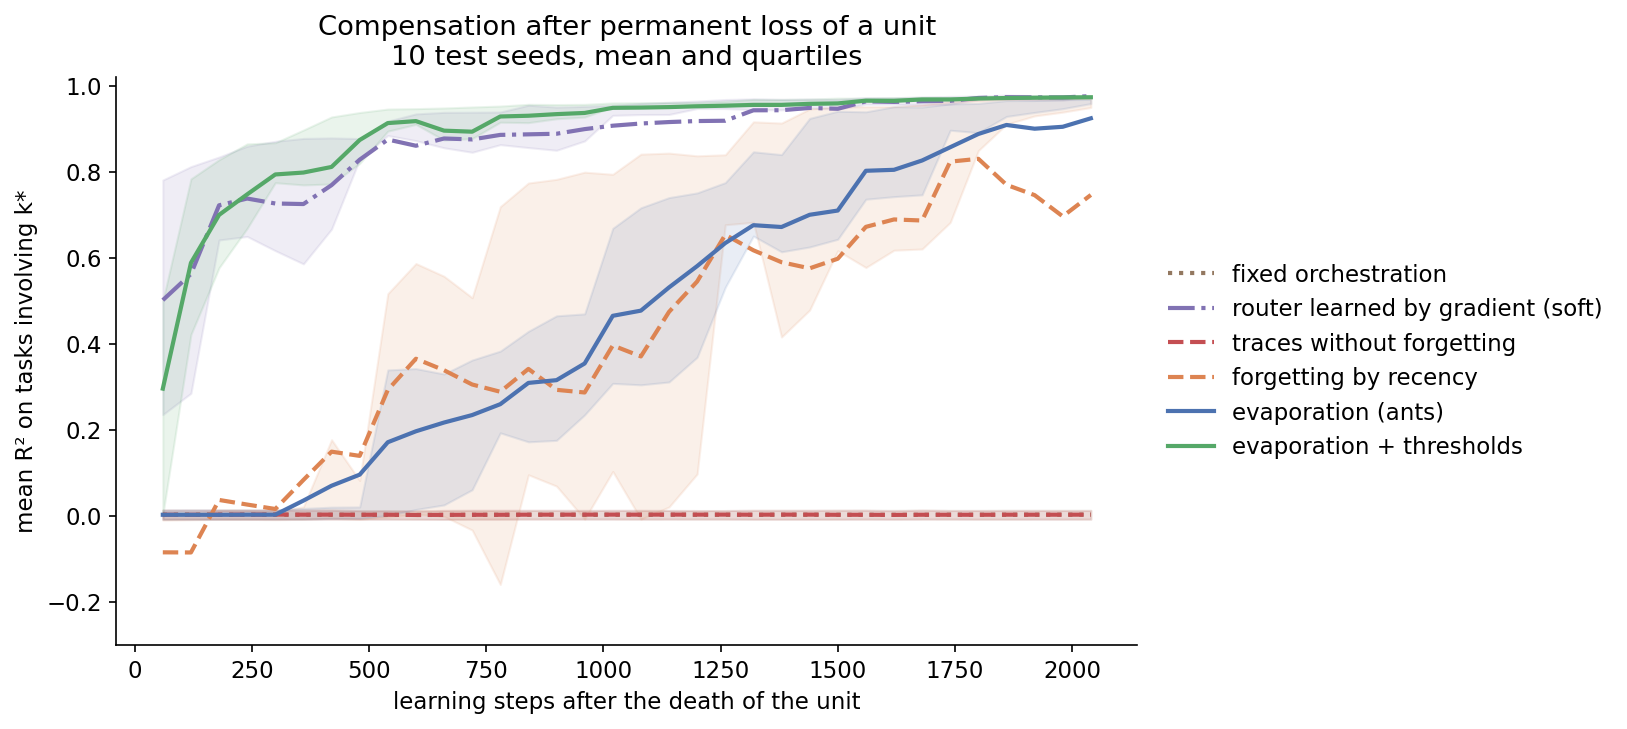
\includegraphics[width=0.95\linewidth]{figures/recovery.png}
\caption{Recovery after the permanent death of the module carrying $k^*$ (Experiment 1, mean and interquartile range over 10 seeds).}
\label{fig:recovery}
\end{figure}

Forgetting enables compensation: evaporation recovers while traces without forgetting and fixed orchestration never do (difference $+0.92$, 10/10 seeds, $p = 0.002$). Alarm and recruitment reduce rerouting latency from about 555 to 4.5 steps and improve recovery (10/10 seeds, $p = 0.002$). At the same rate, time-based evaporation destroys retention ($-0.76$, 10/10, $p = 0.002$). Evaporation beats the monolithic MLP in zero-shot generalisation but not the gradient-trained router ($p = 0.43$), and does not differ from forgetting by recency ($p = 0.56$ and $p = 1.0$). An apparent advantage of the full mechanism over the gradient-trained router (zero-shot 0.88 vs 0.73, 9/10 seeds) was exploratory.

\subsection{Experiment 2: confirmation (seeds 20--29)}

That exploratory advantage was not confirmed on fresh seeds: zero-shot $+0.008$ (95\% CI $[-0.09, +0.09]$, $p = 0.63$) and retention $+0.014$ ($[-0.04, +0.07]$, $p = 0.56$). The first sample was unfavourable to the gradient-trained router (mean retention 0.81 versus 0.88 on the second). With gradients available, the mechanism ties with a gradient-trained router.

\subsection{Experiment 3: no routing gradient (seeds 40--59)}

The routing now receives no gradient. After initial learning, a production phase applies four events: the death of a module; the arrival of two new modules together with another death; a change in the definition of one primitive; and a simultaneous double death. The pool has ten slots, seven occupied at the start, and the system is never told which modules are dead. The main measure, availability, is the mean $R^2$ over the 17 tasks evaluated after every 60-step block of the production phase. A $2\times2$ design crosses the forgetting rule (ema, aco) with the alarm and recruitment (absent, present).

\begin{table}[h]
\centering\small\setlength{\tabcolsep}{5pt}
\begin{tabular}{lcccc}
\toprule
Variant & Availability & Collapses & Final $R^2$ & Final zero-shot \\
\midrule
Recency (ema) & 0.41 & 10/20 & 0.22 & 0.07 \\
Recency + alarm + recruitment & 0.51 & 7/20 & 0.61 & 0.45 \\
Evaporation (aco) & 0.57 & 4/20 & 0.37 & 0.20 \\
Evaporation + alarm + recruitment & 0.76 & 0/20 & 0.60 & 0.39 \\
\bottomrule
\end{tabular}
\caption{Experiment 3, means over 20 seeds. Collapses: seeds with initial retention below 0.5.}
\label{tab:exp3}
\end{table}

The full mechanism beats recency by $+0.35$ ($[+0.29, +0.40]$, 20/20 seeds); the alarm and recruitment add $+0.14$ (18/20, $p = 0.0001$); evaporation beats recency by $+0.21$ (20/20; no sign was predicted). The advantage is not only an initial-learning effect: on the seven seeds where both systems start healthy, the mechanism loses 0.30 of $R^2$ across the events, recency 0.77 (Figure~\ref{fig:availability}).

\begin{figure}[h]
\centering
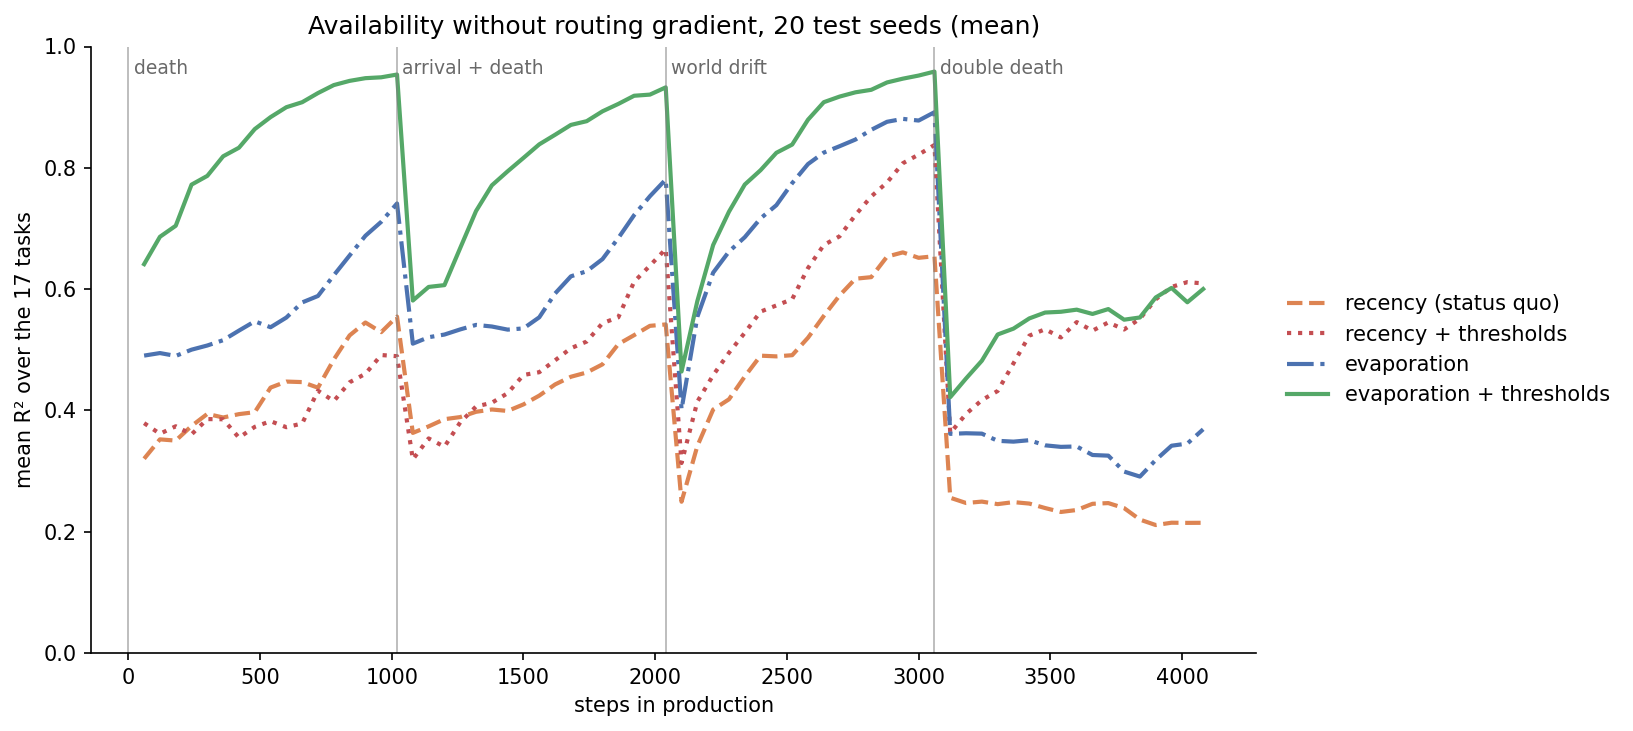
\includegraphics[width=0.95\linewidth]{figures/availability.png}
\caption{Availability during the production phase without routing gradient (Experiment 3, mean over 20 seeds). Vertical lines mark the four events.}
\label{fig:availability}
\end{figure}

\subsection{Experiment 4: standard non-stationary bandits (seeds 80--99; replication 60--74)}

The same scenario is run against SW-UCB, D-UCB and M-UCB, each tuned over its own grid on development seeds. The preregistered thesis that the mechanism beats non-stationary bandits required all three comparisons to succeed.

\begin{table}[h]
\centering\small\setlength{\tabcolsep}{5pt}
\begin{tabular}{lccc}
\toprule
Variant & Availability & Initial $R^2$ & Final $R^2$ \\
\midrule
Evaporation + alarm + recruitment & 0.74 & 0.94 & 0.65 \\
SW-UCB (window 50) & 0.72 & 0.69 & 0.86 \\
D-UCB ($\gamma = 0.98$) & 0.72 & 0.66 & 0.88 \\
M-UCB (change detection) & 0.59 & 0.90 & 0.72 \\
\bottomrule
\end{tabular}
\caption{Experiment 4, main test, means over 20 seeds.}
\label{tab:exp4}
\end{table}

Against SW-UCB the difference is $+0.02$ ($[-0.02, +0.06]$, $p = 0.39$) and against D-UCB $+0.03$ ($[-0.01, +0.06]$, $p = 0.20$): neither is confirmed. Against M-UCB it is $+0.15$ (20/20 seeds). The replication on 15 other seeds shows the same pattern, with the first two differences positive but above the preregistered threshold ($p = 0.03$). The thesis is therefore not retained. The profiles differ: the mechanism learns better initially and absorbs the first events better, whereas SW-UCB and D-UCB recover better late in the run, notably after the double death.

\subsection{Experiment 5: a tuned change-point bandit (seeds 60--79)}

An independent change-point UCB (sliding window, per-arm reset on a quality drop), tuned over 16 configurations, is clearly stronger than recency ($+0.16$, 18/20) but weaker than the mechanism ($0.77$ vs $0.61$, difference $+0.16$, $[+0.11, +0.22]$, 18/20, $p < 10^{-4}$). It learns better initially (0.95 vs 0.91) but loses more across events (0.37 vs 0.21). This is consistent with the result against M-UCB.

\subsection{Experiment 6: ablation (seeds 80--99)}

Recruiting a random available module instead of the least committed one lowers availability from 0.74 to 0.52 ($+0.22$ for least-committed recruitment, $[+0.19, +0.27]$, 20/20). Replacing per-module alarm thresholds with a single collective threshold has no detectable effect ($+0.002$, $[-0.03, +0.03]$, $p = 0.78$). The active ingredient is therefore a piece of collective information, the load of each module in the sense of its total trace, read at the moment of failure. In this scenario all modules are identical, which may explain why individual thresholds bring nothing.

\subsection{Experiment 7: opaque task identifiers (seeds 600--609)}

Each composition now receives only an opaque identifier. The system knows that a path has two slots but not which primitives a task combines; with 8 modules and 12 tasks, success requires discovering that tasks share primitives. After interleaved learning of the 12 known compositions, each of the 8 new compositions is learned for 200 steps from the same state.

\begin{table}[h]
\centering\small\setlength{\tabcolsep}{5pt}
\begin{tabular}{lccccc}
\toprule
Variant & Known & Speed & Final new & Interf. & Align. \\
\midrule
Monolithic MLP & 0.95 & 0.96 & 0.98 & 0.60 & n/a \\
Router trained by gradient & 0.91 & 0.89 & 0.97 & 2.23 & $-8.8$ \\
REINFORCE router & 0.13 & 0.29 & 0.50 & 0.21 & $-0.24$ \\
Evaporation + alarm + recruitment & 0.21 & 0.29 & 0.55 & 0.21 & $-0.20$ \\
\bottomrule
\end{tabular}
\caption{Experiment 7, means over 10 seeds. Known: $R^2$ on the 12 known tasks. Speed: mean $R^2$ on a new task over 10 evaluations during 200 steps. Final new: $R^2$ on the new task at the end. Interf.: drop of mean $R^2$ on the known tasks. Align.: best $R^2$ of any module approximating each primitive, averaged over primitives.}
\label{tab:exp7}
\end{table}

The mechanism learns new compositions far more slowly than the monolithic MLP and the gradient-trained router (0/10 seeds, $p = 0.002$) and ties with the REINFORCE router. Its lower interference is not a virtue, since little was learned in the first place. No variant aligns its modules with the primitives: none discovers the decomposition. The MLP and the gradient-trained router learn each task as its own function and overwrite previous ones, an instance of catastrophic interference \citep{mccloskey1989catastrophic}. These failures were visible on the development seeds and were declared in the preregistration before the test.

\subsection{Experiment 8: sparse top-$k$ mixtures of experts (seeds 700--719)}

This experiment and the next were run after a first version of this manuscript. In the protocol of Experiment~1, the mechanism faces routers trained by gradient with noisy top-$k$ gating, per task symbol. The noise scale and an optional balancing loss were tuned on development seeds. As declared in the preregistration, two opponents were kept after seeing the tuning results, because the best top-1 configuration never recovers from the loss of a module, which would have made the compensation comparison trivial.

\begin{table}[h]
\centering\small\setlength{\tabcolsep}{5pt}
\begin{tabular}{lccc}
\toprule
Variant & Retention & Zero-shot & $k^*$ tasks, recovered \\
\midrule
Evaporation + alarm + recruitment & 0.89 & 0.87 & 0.97 \\
Top-1 (noise 0.3, balancing 0.01) & 0.96 & 0.95 & 0.05 \\
Top-2 (noise 0.3) & 0.93 & 0.89 & 0.96 \\
\bottomrule
\end{tabular}
\caption{Experiment 8, means over 20 seeds.}
\label{tab:exp8}
\end{table}

Against top-2, the mechanism is behind in zero-shot generalisation ($-0.03$) and retention ($-0.04$), not significantly at the preregistered threshold ($p = 0.009$ and $0.012$ against $0.0083$), and ahead in recovery by a negligible $+0.011$ (18/20, significant). Against top-1, it is clearly behind in zero-shot generalisation ($-0.08$) and retention ($-0.07$), and far ahead in recovery ($+0.93$, 20/20): a top-1 router cannot reroute once its selected module is dead. With gradients available, the mechanism brings no learning advantage.

\subsection{Experiment 9: heterogeneous modules (seeds 720--739)}

The production scenario of Experiment~3 is rerun with heterogeneous modules: their hidden sizes are 2, 4, 8, 16, 32, 64, 2, 4, 8 and 16 units, in a seed-dependent order, so that a little-used module may be little used because it is weak. The bandits keep the configurations of Experiment~4, as preregistered; nothing is tuned.

\begin{table}[h]
\centering\small\setlength{\tabcolsep}{5pt}
\begin{tabular}{lcccc}
\toprule
Variant & Availability & Initial $R^2$ & Collapses & Final $R^2$ \\
\midrule
Evaporation + individual thresholds & 0.72 & 0.89 & 0/20 & 0.55 \\
Evaporation + collective threshold & 0.72 & 0.89 & 1/20 & 0.53 \\
SW-UCB (window 50) & 0.71 & 0.75 & 2/20 & 0.76 \\
D-UCB ($\gamma = 0.98$) & 0.68 & 0.63 & 7/20 & 0.74 \\
\bottomrule
\end{tabular}
\caption{Experiment 9, means over 20 seeds.}
\label{tab:exp9}
\end{table}

Individual thresholds still bring nothing ($+0.002$, $[-0.02, +0.03]$, $p = 0.93$), contrary to the hypothesis that heterogeneity would make them useful. The mechanism ties with SW-UCB ($+0.01$, $p = 0.90$) and is ahead of D-UCB ($+0.04$, $[+0.01, +0.07]$, 16/20, $p = 0.014$). That last edge should not be read as structural: the bandits were tuned for homogeneous modules, and D-UCB collapses at initial learning on 7 of 20 seeds. The profiles of Experiment~4 persist, with better initial learning for the mechanism and better final recovery for the bandits.

\subsection{Experiments 10 and 10b: oracle local credit (seeds 800--809 and 810--819)}

The diagnosis of Experiment~7 is put to the test in the same opaque-identifier world. An oracle gives each slot of the path its own local quality: slot 1 is compared with the true intermediate $P_i(x)$, slot 2 with $y$. Level 1 uses the local quality for traces and alarms only, modules still learning on the global loss; level 2 also gives each module its own learning target. Experiments 10 and 10b are two independent implementations of this design, written without knowledge of each other (Section~\ref{sec:integrity}) and differing slightly in the oracle for slot 2; on three shared seeds the reference values are identical and the local variants agree within 0.04, except one known-task value that differs by 0.10 (seed 802). Experiment 10b adds a dense gradient router given the same local losses.

\begin{table}[h]
\centering\small\setlength{\tabcolsep}{5pt}
\begin{tabular}{llcccc}
\toprule
Exp. & Variant & Known & Speed & Interf. & Align. \\
\midrule
10 & Reference (global credit) & 0.18 & 0.31 & 0.21 & $-0.24$ \\
10 & Level 1: local credit, routing only & 0.09 & 0.22 & 0.19 & $-0.27$ \\
10 & Level 2: local credit, routing + content & 0.97 & 0.94 & 0.20 & 0.99 \\
10b & Reference & 0.20 & 0.30 & 0.22 & $-0.28$ \\
10b & Level 2 & 0.97 & 0.95 & 0.16 & 0.99 \\
10b & Dense gradient router, local losses & 0.99 & 0.95 & 0.66 & $-1.65$ \\
\bottomrule
\end{tabular}
\caption{Experiments 10 and 10b, means over 10 seeds each. Columns as in Table~\ref{tab:exp7}.}
\label{tab:exp10}
\end{table}

Local credit for routing alone makes things worse (known tasks $-0.09$ and speed $-0.09$, 0/10 seeds each): the traces favour modules that resemble primitives while the global loss trains them towards something else. Level 2 learns the new compositions far faster than the reference ($+0.63$, 10/10 in Experiment~10; $+0.65$, 10/10 in 10b), with modules aligned with the primitives. Given the same local losses, the dense gradient router ties on speed ($-0.008$, $p = 0.85$) but smears the modules (alignment $-1.65$ vs $0.99$, 10/10) and interferes with the known tasks (0.66 vs 0.16, 10/10). The lock of Experiment~7 was therefore the learning signal of the modules, not an inability of the traces to find a path once modules are correct.

\subsection{Experiment 11: sparse routers with local losses (seeds 820--829)}

Is the clean decomposition of 10b a property of traces or of hard assignment in general? Top-1 and top-2 routers, with the configurations of Experiment~8 and the same local losses, are compared with trace routing. The prior stated before the experiment gave a 60\% chance that a sparse router would align as well; after the development seed it was revised to 35\%, as recorded in the preregistration.

\begin{table}[h]
\centering\small\setlength{\tabcolsep}{5pt}
\begin{tabular}{lcccc}
\toprule
Variant & Known tasks & Speed on new & Interference & Alignment \\
\midrule
Trace routing, local losses & 0.97 & 0.95 & 0.19 & 0.99 \\
Top-1 router, local losses & 0.97 & 0.66 & 0.28 & 0.46 \\
Top-2 router, local losses & 0.99 & 0.87 & 1.21 & 0.94 \\
\bottomrule
\end{tabular}
\caption{Experiment 11, means over 10 seeds.}
\label{tab:exp11}
\end{table}

Neither sparse router matches the traces. Top-1 gating learns new compositions slowly ($-0.29$ vs traces, 10/10) and aligns modules only partially ($-0.53$, 10/10), with no significant difference in interference. Top-2 gating aligns almost as well ($-0.05$, 10/10) but interferes far more (1.21 vs 0.19, 10/10) and learns somewhat slower ($-0.08$, 10/10). The combination of fast learning, clean alignment and low interference is specific to the trace rule among the routers tested.


\section{Beyond the toy world: preservation, modular JEPA, and a continual world model}
\label{sec:beyond}

The experiments of this section were run after the ones above, each preregistered before its test seeds; the preregistrations, with the development runs they declare, are in the repository.

\subsection{Experiments 14 to 16b: does the mechanism preserve a function?}

A reviewer asked whether the traces select important skills or merely frequently solicited ones. We made one primitive rare (its tasks sampled with relative weight 0.02) in the production world of Experiment~3, killed the module carrying a frequent primitive, and measured the rare skill before and after. Experiment~14 had three protocol flaws found by an external review (reserve modules active from the start, recruitment rules acting during initial learning, recruitments counted from the start); it is kept with its flaws recorded and was redone as Experiment~14b on a common-state harness: one model learned up to the event and deep-copied before every condition, production data drawn once and shared, recruitments timestamped.

\begin{table}[h]
\centering\small\setlength{\tabcolsep}{4pt}
\begin{tabular}{llcccc}
\toprule
Capacity & Rule & Avail. & Rare before & Rare after & Killed recov. \\
\midrule
none (5 active) & least comm. & 0.46 & 0.89 & $-0.54$ & 0.59 \\
none & random & 0.41 & 0.89 & $-0.33$ & 0.54 \\
none & none & 0.47 & 0.89 & $-0.54$ & 0.58 \\
spare (7 active) & least comm. & 0.76 & 0.59 & 0.61 & 0.92 \\
dormant (5+2 held) & least comm. & 0.87 & 0.89 & 0.92 & 0.96 \\
\bottomrule
\end{tabular}
\caption{Experiment 14b, seeds 1400--1409, means over 10 seeds.}
\label{tab:exp14b}
\end{table}

With no spare capacity the recruitment rule changes nothing ($-0.01$ on availability, $p = 0.77$): the rare skill collapses with and without recruitment, consumed by exploration itself, and the first post-event recruit is the rare specialist in 3/10 seeds (random: 2/10). Held-back reserves preserve it (0.89 to 0.92) and recover the killed function; spares active from the start preserve what they had but had learned the rare skill less well (0.59), because they dilute exploration during learning. Experiment~15b (identical relearning streams) found that a consumed specialist relearns its function no faster than a fresh module ($+0.06$ on the area under the learning curve, $p = 0.32$), and that a module repurposed to another function relearns slower than a fresh one ($-0.20$, 0/10, $p = 0.002$). Experiment~16b found no gain from resetting a recruited module's optimizer state ($-0.01$) or its weights ($-0.06$, 1/10). A perturbed replay of all 110 runs of 14b/16b (initial weights perturbed by $10^{-6}$) left the six preregistered decisions unchanged while individual runs moved, which is why we read these results at the level of the aggregate.

\subsection{Experiments 12 and 13: competing JEPA predictors}

In a sequential world with five unnamed primitives that persist for a few steps and eight noise channels per observation, a tiny JEPA (shared encoder, EMA target) hosts competing predictors assigned by hindsight error, as in COMET \citep{comet2024} and MOSAIC \citep{mosaic2001}, against an attention-based assignment in the style of Recurrent Independent Mechanisms \citep{goyal2021rim}. Competition reaches a module purity of 0.84 against 0.36 for attention-based assignment (5/5 seeds); the prior over the winner needs memory, not the current state (after a switch to a held-out pair, a persistence prior recovers to 0.05 where a state classifier stays at 1.52); traces tie with plain persistence ($+0.002$). When a sixth primitive appears, surprise-triggered recruitment of a dormant reserve instantiates a new predictor without degrading the old ones (error on the new primitive 0.49 vs 0.68 for fixed competition, 5/5), but no better than competition merely over-provisioned with three extra modules (differences of 0.002 and 0.001).

\subsection{Experiment 17: continual dynamics on LeWorldModel's frozen representation}
\label{sec:exp17}

LeWorldModel \citep{lewm2026} is a JEPA world model trained end to end from pixels. We kept the released encoder and projector for Two-rooms frozen, cached the 192-dimensional embeddings of all 920,809 frames of its dataset (parity with the model's own encoding exact in fp32), and trained predictors with LeWorldModel's own architecture on windows aligned with its configuration (history 3, frameskip 5, action blocks of 5). Regime A is the original dynamics; regime B uses the same images with the action vector rotated by $90^\circ$, so that a regime can be inferred only from prediction errors, never from appearance. The stream has three phases of 1500, 1500 and 500 steps of four episodes: A, then B with A at 2\%, then A again. Measures are relative five-step latent errors on held-out episodes; access error uses the module chosen before observing the outcome. Three development runs on one seed, declared in the preregistration, set the banks' thresholds (freezing at 0.1, surprise at four times the recent error after a warm-up, a 100-step cooldown); the replay buffer was not tuned.

\begin{table}[h]
\centering\small\setlength{\tabcolsep}{4pt}
\begin{tabular}{lccccc}
\toprule
System & A, P1 & A during B & B, P2 & A, P3 & B, P3 \\
\midrule
single predictor & 0.070 & 1.60 & 0.063 & 0.058 & 1.68 \\
single + replay (20k windows) & 0.064 & 0.131 & 0.080 & 0.072 & 0.107 \\
bank, persistence prior & 0.108 & 0.132 & 0.116 & 0.111 & 0.138 \\
bank, traces + recruitment & 0.108 & 0.132 & 0.116 & 0.111 & 0.138 \\
\bottomrule
\end{tabular}
\caption{Experiment 17, five seeds; standard deviations between 0.002 and 0.047. The banks use twice the forward passes.}
\label{tab:exp17}
\end{table}

The banks behaved as designed on every seed (the A specialist froze before B, one surprise, one activation, no recruitment) and are identical to the fourth decimal, the prior having nothing to decide with one module per regime. Against replay they are not better on any retention measure (A during B: $+0.000$, 2/5; B at the end: $+0.031$, 0/5; A at the end: $+0.039$, 0/5), and they cap A at the level where it froze. By the preregistered stop rule, the trace and recruitment line stops for continual world models.

\section{A training defect, a Two-rooms planning gain, and its failure on PushT}
\label{sec:gap}

\subsection{The gap and its cause}

The retrained predictor stack (action encoder, predictor, projection head, instantiated from the released configuration at random init and trained 8 epochs on the frozen embeddings) reaches a relative five-step latent error of 0.006 on held-out windows of three real frames, against 0.067 for the released predictor. With the authors' evaluation script unchanged, on 100 episodes each, the released model succeeds in 85 (exact 95\% interval 77 to 91) and the retrained one in 36 (27 to 46). Six diagnostics, each a small kernel on a free GPU and each starting from three real frames, failed to explain it: action normalisation (no effect); one-step error on 8,500 windows of random actions played in the environment (both degrade to about 0.55 to 0.60); open-loop rollouts over ten horizons (the retrained predictor better throughout); ranking of 19 random candidate plans from 40 cloned starts (Spearman 0.98 vs 0.90 in its favour); the 100 evaluation episodes split by whether the goal lies across the wall (the gap as large within a room, 40\% vs 90\%); and hand-designed straight and self-cancelling action sequences from cloned starts (the retrained predictor more accurate, 39/40 starts). Instrumenting the evaluation loop showed what the retrained model's plans did: approach the goal half as fast, move away from it on 49\% of steps, with plans whose consecutive blocks were nearly orthogonal. With the authors' solver reproduced from 30 cloned starts, the plan it selected was predicted by the retrained model to cost 0.68 and cost 37.0 in truth (per-start median ratio 27.5), against 12.4 and 43.8 for the released model (median 1.5). A later control showed that most of this apparent optimism is an artefact of the measurement: the solver searches unbounded normalised actions and reports the cost of the unclipped plan, while the environment executes the plan clipped to its bounds (13\% of action components saturated for the neural predictors, 24\% for the bilinear one); re-predicting the cost of the clipped plan brings the median ratio of true to predicted cost to 0.8 for the released predictor, 1.5 for the corrected neural one (18 unclipped) and 1.3 for the bilinear one (1.6 unclipped). This control was run on the corrected network, not on the defective checkpoint whose ratios of 27.5 and 13.1 are quoted above, so those earlier ratios are not quantitatively attributed to clipping; it shows that the mismatch between evaluated and executed actions accounts for most of the apparent optimism in the predictors it tested, and it neither establishes an absence of exploitable errors nor says what a solver constrained during its search would select, since re-predicting after the fact does not change the chosen plan.

The cause was found by an external reviewer reading the training recipe rather than measuring outputs. Our loss supervised only the last prediction of a context of three real frames; the official loss supervises every position; and the official planner starts an episode from a single frame, feeding the predictor contexts of one, two and then three observations, the later ones partly its own predictions. Measured on held-out windows, the retrained network's relative error was 1.18 at a context of one frame and 1.03 at two, against 0.006 at three; the released predictor's was 0.066 at every length. Every diagnostic above had started from three real frames and could not see this. A variant retrained with the official loss, everything else equal, has an error of 0.005 at every context length and plans like the released predictor: 84, 85, 89 and 81 on evaluation seeds 42 to 45 against 85, 83, 87 and 80, with balanced discordant episodes (5/6, 4/2, 6/4, 7/6). The gap was an artefact of our recipe. What remains of it is a methods result: a predictor can be far more accurate on every offline measure a study constructs and fail where the planner actually calls it, and the way to find such a defect was to compare the recipe, not the outputs.

\subsection{Experiment 18: a bilinear predictor in place of the released one}
\label{sec:operator}

We fitted, by ridge least squares on the training windows of the cache (one minute on a free GPU, no neural training), a predictor of the embedding five frames ahead that is linear in the last three embeddings and in the 10-dimensional action block, and bilinear in the current embedding and the action block: 2,507 coefficients per output dimension. Its relative one-step latent error on held-out windows is 0.69, ten times the released predictor's, and 0.66 and 0.68 at contexts of one and two frames, so it shows none of the short-context error explosion of the defective recipe. The exploratory run on the authors' evaluation seed gave 97/100; the confirmation was preregistered with four hypotheses before any further run. The official evaluation samples starts and goals from the whole dataset, not from the episodes held out for the latent error, and the four seeds are evaluation seeds of one fitted predictor, not independent fits.

\begin{table}[h]
\centering\small\setlength{\tabcolsep}{5pt}
\begin{tabular}{lccccc}
\toprule
Predictor & latent error & seed 42 & seed 43 & seed 44 & seed 45 \\
\midrule
released (end-to-end) & 0.067 & 85 & 83 & 87 & 80 \\
retrained, loss on the last position only & 0.006 & 36 & & & \\
retrained, official loss (every position) & 0.005 & 84 & 85 & 89 & 81 \\
bilinear (ridge least squares) & 0.69 & 97 & 99 & 100 & 96 \\
linear only & 0.83 & 57 & & & \\
bilinear, current embedding only & 0.69 & 96 & & & \\
bilinear, ridge $\times 10$ / $\div 10$ & 0.70 / 0.69 & 96 / 97 & & & \\
\bottomrule
\end{tabular}
\caption{Experiment 18: planning success on Two-rooms (100 episodes per seed, authors' evaluation script unchanged) and relative one-step latent error on held-out windows of three real frames. Exact 95\% intervals: 90 to 100 for the bilinear predictor's four seeds, 71 to 93 for the released predictor's, 72 to 94 for the corrected neural predictor's.}
\label{tab:exp18}
\end{table}

K1 held: the bilinear predictor is above the released one on all three fresh seeds, with every discordant episode in its favour (16/0, 13/0, 16/0). It is also above the neural predictor retrained with the official loss on all four seeds, with discordant episodes 15/2, 14/0, 11/0 and 16/1 (exact McNemar $p \le 0.002$ on each seed), so the comparison no longer depends on a defective neural baseline. K2 held as written, with a reading narrower than the hypothesis suggested: in the exploitation probe (goals from random plans, contexts of three real frames, a different protocol from the official evaluation), the per-start median ratio of true to predicted cost is 1.6 for the bilinear predictor, 1.5 for the released one and 13.1 for the defective retrained network in this run; but the bilinear predictor also predicts much higher costs (57.7 against 11.8), its absolute optimism gap is comparable to the others' (27 against 26), its executed plans cost more than the released model's on 25 of 30 starts, and the action-bounding control above shows that, for the predictors it tested, these ratios mostly measure clipping. In that same probe the corrected neural predictor reaches the lowest true cost of the three (23.7 against 37.7 and 84.8): the probe did not reproduce the ranking of the three predictors in the official evaluation. A low ratio with a high denominator establishes neither better plans nor an absence of exploitation. K3 held for the linear ablation (57\% without the bilinear terms, 42 discordant episodes in favour of the bilinear predictor against 2) and not for history: removing it changed the score little on that seed (96\%), which is not evidence of equivalence. K4: ridge $\times 10$ and $\div 10$ gave 96 and 97 on that seed. The defensible statement: on this Two-rooms evaluation, three predictors on one encoder with held-out latent errors of 0.005, 0.067 and 0.69 plan at about 85, 84 and 98; this bilinear predictor improves planning despite a higher held-out latent error, the tested ablations support a contribution from the bilinear state-action terms, and the mechanism behind the advantage is not established. Experiment~19 tests the same fitting recipe on the second task of the release; its negative result below limits the observed planning advantage to Two-rooms.

\subsection{Experiment 19: the fixed recipe underperforms on PushT}
\label{sec:pusht}

The protocol was fixed and published before the PushT cache, fitting or evaluation. It specifies the released PushT checkpoint (revision \texttt{22b330c28c27}), dataset archive (\texttt{655cd446b992}), evaluation code (\texttt{8edfeb336732}) and \texttt{stable-worldmodel} version 0.1.1. We cached the frozen encoder's 192-dimensional embeddings and independently checked preprocessing parity against the pinned official evaluation transform on 64 frames. The maximum absolute difference was $3.20\times10^{-6}$, below the $10^{-5}$ tolerance fixed before that check. A split by episode, with seed 0, holds out 10\% for latent-error measurement. The bilinear features, ridge coefficient $10^{-2}N$, three-frame history and five-frame action blocks are unchanged from the specified recipe, with no parameter tuning. The neural reference is freshly initialised with training seed 1 and trained for eight epochs with every position supervised. Each task uses its own released encoder and a new fit: this tests transfer of the recipe, not transfer of Two-rooms weights.

The pinned official evaluator runs 100 tasks per model on each evaluation seed 42--45, with horizon 5, action blocks of 5, receding horizon 5, execution budget 50 and goal offset 25. The solver, action bounding, preprocessing, starting-task selection and success criterion are unchanged. Hooks only select the saved predictor, assert settings and normalisation, record results, and give each run a distinct video directory. Every predictor receives identical ordered episode/start/goal tuples within each seed. As on Two-rooms, evaluation tasks come from the whole dataset, including training episodes; the held-out split applies to the latent-error tables, not to planning. Four evaluation seeds do not constitute four independently trained predictors. The paper's published PushT reference uses a different protocol and is not the comparator for this test.

The primary criterion is strictly more bilinear successes than released successes on each of seeds 43, 44 and 45; a tie fails it. Seed 42 is exploratory. The comparison to the correctly retrained network is secondary and separately evaluated. All twelve runs completed. Tables~\ref{tab:exp19}--\ref{tab:exp19paired} are generated from the archived individual outcomes and context-error measurements, with the score totals, task identities and exact paired tests recomputed by \texttt{tools/analyze\_exp19.py}.

% Generated by tools/analyze_exp19.py; do not edit by hand.
\begin{table}[htbp]\centering\small
\begin{tabular}{lrrrrr}\toprule
Predictor & seed 42 & seed 43 & seed 44 & seed 45 & Mean (\%) \\\midrule
Released & 89 & 86 & 89 & 85 & 87.25 \\
Retrained, official loss & 93 & 94 & 91 & 89 & 91.75 \\
Bilinear, ridge & 35 & 40 & 39 & 36 & 37.50 \\
\bottomrule\end{tabular}
\caption{Experiment 19: PushT successes out of 100 matched tasks per evaluation seed. Seed 42 is exploratory; seeds 43--45 determine the preregistered verdict. Means are descriptive across all four evaluation seeds of one fitted predictor of each type.}
\label{tab:exp19}\end{table}
\begin{table}[htbp]\centering\small
\begin{tabular}{lrrr}\toprule
Predictor & context 1 & context 2 & context 3 \\\midrule
Released & 0.00803 & 0.00792 & 0.00831 \\
Retrained, official loss & 0.00355 & 0.00350 & 0.00365 \\
Bilinear, ridge & 0.08201 & 0.06799 & 0.06820 \\
\bottomrule\end{tabular}
\caption{Experiment 19: relative one-step latent errors on held-out PushT episode windows at each context length. Unlike Two-rooms, the bilinear predictor has both higher errors and lower planning success than the neural predictors.}
\label{tab:exp19context}\end{table}
\begin{table}[htbp]\centering\small
\begin{tabular}{rlrrr}\toprule
Seed & Reference & $b/c$ & $\Delta$ (points) & Exact $p$ \\\midrule
42 & Released & 2/56 & -54 & $1.19\times10^{-14}$ \\
42 & Retrained, official loss & 1/59 & -58 & $1.06\times10^{-16}$ \\
43 & Released & 3/49 & -46 & $1.04\times10^{-11}$ \\
43 & Retrained, official loss & 1/55 & -54 & $1.58\times10^{-15}$ \\
44 & Released & 3/53 & -50 & $8.14\times10^{-13}$ \\
44 & Retrained, official loss & 4/56 & -52 & $9.08\times10^{-13}$ \\
45 & Released & 2/51 & -49 & $3.18\times10^{-13}$ \\
45 & Retrained, official loss & 2/55 & -53 & $2.30\times10^{-14}$ \\
\bottomrule\end{tabular}
\caption{Experiment 19: paired comparisons of the bilinear predictor to each reference. $b$ counts tasks only the bilinear predictor solves; $c$ counts tasks only the reference solves. $\Delta$ is bilinear minus reference success. The exact two-sided McNemar tests are reported per seed without pooling repeated evaluations into independent training runs.}
\label{tab:exp19paired}\end{table}


The primary criterion fails on all three confirmatory seeds: the bilinear predictor loses 46, 50 and 49 percentage points to the released predictor, and 54, 52 and 53 to the retrained network. This is a large performance loss, not an equality near a ceiling. On seed 43, for example, only 3 tasks are solved exclusively by the bilinear predictor whereas 49 are solved exclusively by the released one. In the preregistered wording, superiority is not confirmed on PushT with this recipe; the observed direction is consistently the opposite. The corrected neural predictor has the highest observed score on each evaluation seed, a descriptive comparison that was not the primary hypothesis.

The bilinear predictor has higher latent error at each context length and lower planning success than both neural references. Thus the reversed error/success ranking observed on Two-rooms does not recur on PushT. The experiment does not identify why the recipe fails here. Contact dynamics, the learned coordinates, model capacity, regularisation and interaction with the fixed planner are candidate explanations, not conclusions of this comparison. No post-result adjustment or additional search is included in Experiment~19. The fixed-recipe series closes with a Two-rooms gain and a PushT loss.

\section{Discussion}

\paragraph{What the mechanism is.} Across experiments, the mechanism behaves as a coordination and resilience device. It needs forgetting, and at the rate tested, forgetting tied to solicitation: time-based evaporation at the same rate erases routes for symbols that are simply not being used, while a much slower time-based rate was not tested. Its resilience comes from recruiting the least committed module, which avoids disturbing specialists; this echoes the reallocation of idle workers in insect societies \citep{bonabeau1996threshold,krieger2000robots}. The individuality of alarm thresholds, which was one of the starting intuitions, is not supported, with homogeneous or heterogeneous modules. A reading in terms of local traces in normal operation and a collective quantity consulted only under exception fits the ablation, but remains an interpretation.

\paragraph{What it is not.} It is not better than the best standard non-stationary bandits, which come with theoretical guarantees \citep{garivier2011switching}, and it does not beat routers trained by gradient when gradients are available, whether dense or sparse; its only clear advantage there is over top-1 routing after a module dies. It does not discover structure on its own. The explanation, tested in Experiments 10 to 11, is the learning signal of the modules: the quality of a whole path is not noisy but conjunctive, staying near zero until both modules are right at once, so modules never become primitives, and traces indexed by opaque identifiers have nothing consistent to route to. Giving each module an exact local error settles it: with local errors, traces find the shared primitives across opaque tasks, and do so with a cleaner decomposition and less interference than dense or sparse gradient routers given the same local losses. The remaining question is where a module's local error can come from without an oracle; a module that predicts in a latent space supplies its own. Modules with their own local prediction error, for instance predictors trained in a latent space, would supply the missing signal. The difficulty of learning module layouts reported by \citet{bahdanau2019systematic} points in the same direction.

\paragraph{What it does not protect.} Experiments 14b to 16b add a limit that no earlier experiment could show: nothing in the mechanism protects a function in use. Recruitment and exploration both consume a specialist once spare capacity is gone, a consumed specialist is worth no more than a fresh module, and resetting a recruited module does not help. Protection, where it was observed, came from capacity held back until an event. The mechanism allocates work; it does not preserve functions, and nothing in it distinguishes a rarely used function from a dispensable one, which is the distinction a reviewer's question about rare but critical skills brought out.

\paragraph{Against replay, and what the planning gap says about our own measures.} On a released world model, under changing dynamics, the mechanism's one structural asset, instantiating a new predictor on surprise without touching the old ones, worked as designed and was not worth more than a reservoir replay buffer with no tuned parameter. We stopped the line by the rule written before the pilot. The planning gap of Section~\ref{sec:gap} then qualifies the whole continual study: all its retention measures are in-distribution latent errors, and we now have a case where such errors, refined in every way we could think of, failed to predict control. The honest scope of Experiment~17 is therefore retention of prediction, not retention of control, and the design note's planning phase, which we did not reach, is where the question should be settled.

\paragraph{What the two planning tasks establish.} On Two-rooms, the correctly retrained, released and bilinear predictors have held-out latent errors of 0.005, 0.067 and 0.69 and average planning successes of 84.75\%, 83.75\% and 98.00\%. Average latent error therefore does not rank these three predictors in that evaluation. On PushT, the bilinear recipe instead has both higher error and much lower success, averaging 37.50\% against 87.25\% for the released predictor and 91.75\% for the corrected network. This bounds the Two-rooms finding; it does not establish that prediction accuracy is generally irrelevant, that bilinear operators generally plan better, or that either error ordering gives a universal ranking rule. The separate exploitation probe also failed to reproduce the official Two-rooms ranking and establishes no immunity to exploitable model errors.

The bilinear predictor is a regression on learned observables. Its relation to the Koopman view of dynamics, in which linear predictors on lifted observables serve model predictive control \citep{korda2018koopman} and bilinear realisations are preferred for control-affine systems \citep{bruder2020bilinear}, is a connection to existing work, not a demonstrated mechanism: closure of these observables under the operator was not shown on either task. The value-equivalence principle \citep{grimm2020value}, that a model need only preserve what matters to the planner, motivates measuring control directly. It does not explain this experiment's task-dependent outcome. The contribution is a paired comparison on two released world models, including a failed extension, together with a documented training defect that six offline diagnostics missed.

\paragraph{Limitations.} Experiments 1 to 16b come from a single toy world (five primitives in dimension 8); Experiments 12, 13 and 17 from one sequential world and one released model on one environment, with five seeds each, so their results are effect sizes with per-seed values rather than tests. The production scenarios were designed to probe resilience and are not neutral. Opponents received modest tuning budgets (8 to 20 configurations on three seeds), contextual bandits are not among them, and in Experiment~9 the bandits were not re-tuned for heterogeneous modules. Heterogeneity was limited to module size; costs, latencies and partial failures were not modelled. The decomposition of tasks is given in Experiments 1 to 6, and the local errors of Experiments 10 and 11 come from an oracle, which amounts to supervising the decomposition. Sparse routers in Experiment~11 kept the configurations of Experiment~8, not re-tuned for local losses. The initial modules are supervised regressors; later JEPA experiments and visual world-model evaluations also remain in simulation. Experiments 18 and 19 cover only two tasks, one released encoder and one fitted predictor per model type per task, with planning starts drawn from the full fitting dataset. They do not measure generalisation to disjoint planning episodes, independent retraining seeds or physical systems. The PushT recipe was deliberately not tuned, so its failure does not rule out other bilinear representations or training choices. A regime in which commitment-based recruitment beats sliding-window and discounted UCB, for example with frequent failures and scarce reserves, with opponents re-tuned for that regime, remains to be identified.

\section{Research integrity statement}
\label{sec:integrity}

\paragraph{Development seeds.} Every test used seeds separate from those used to check code and tune opponents. What development runs revealed is stated in the preregistrations, including the expected failures of Experiment 7.

\paragraph{A protocol found after the fact.} While preparing publication, the files of a preregistered protocol (Experiment 4) were found in the execution environment. They came from an earlier execution that is absent from the history of the conversation that produced the rest of this work, and the protocol had not been reported. Its code hashes match its preregistration. Its main test had stopped at 15 of 20 seeds; seeds 95 to 99 were completed with the same code before any analysis. It is reported here in full, although it weakens an earlier claim.

\paragraph{Seed reuse.} The preregistrations of Experiments 5 and 6 state that their seeds had never been used. Seeds 60 to 74 and 80 to 99 had in fact been used by Experiment 4. No decision depended on those results, which were unknown at the time, and the code is deterministic: the mechanism produces bit-identical results on the 20 seeds shared by two independent runs. The statement was nevertheless false, and corrections are attached to the published preregistrations.

\paragraph{A second set of files from an unseen execution.} After the first version of this manuscript, the preregistrations and code of Experiments 8 and 9, the completed test runs of Experiment~8 and the beginning of a third, unpreregistered experiment were again found in the execution environment, from an execution absent from the conversation history. The quoted code hashes match, and the preregistrations were written before the test runs. Experiment~8 was analysed and Experiment~9 was run according to their written protocols; the third experiment was not continued and is kept as a marked draft.

\paragraph{A third set of files, and an overwrite.} Experiment~10 (preregistration, code, complete test runs and a commit) was found in the execution environment while a second implementation of the same design was being written without knowledge of it. The second implementation briefly overwrote the first's preregistration and code, which were restored byte for byte from the commit, and was then kept as Experiment~10b on fresh seeds.

\paragraph{Cause of the unseen executions, and later incidents.} The files found three times came from attempts of the same conversational turns that the chat interface reported as failed while their tools kept running in the shared environment; Experiments 12 and 13 were produced the same way and completed with the same code where the attempts were cut. Later, an external review of the repository found four protocol flaws (a seed reset that did not reach the world's own generator, recruitment rules acting before the event they were meant to answer, recruitments counted from the start of learning, reserves that were active rather than dormant) and one false claim of compute savings; each is recorded next to the result it affects, and the affected experiments were redone (15b, 14b, 16b) rather than edited. A reviewer's non-reproduction of one run led to a perturbed replay of all 110 runs of 14b/16b: the preregistered decisions are unchanged, individual trajectories are chaotic under alarms and sampled routing. The last incident is the one of Section~\ref{sec:gap}: a planning gap we had declared unexplained after six diagnostics was explained by an external reviewer who compared our training loss with the official one; we had measured outputs where the defect was in the recipe, and we had written that the obvious causes were excluded. That sentence was withdrawn.

\paragraph{Experiment 19 execution and reporting.} The preregistration remains unchanged. The cache retry changed extraction storage after a disk constraint, not the dataset or model. Independent cache parity was checked before fitting; the full eight-epoch checkpoint was used without selecting an epoch from planning outcomes. All twelve planning runs, including the failed primary and secondary comparisons, are archived with matching task identities, model hashes and a completion manifest. Historical results of the earlier experiments were not rerun or replaced.

\paragraph{Provenance check.} A script in the repository recomputes every code hash quoted in the preregistrations and prints a ledger of seeds per result file with all overlaps between test seeds of different experiments. Quoted source hashes are recoverable from the working tree or Git history. The current wrappers for Experiments 17 and 18 differ from their preregistered versions: the former changed the default run mode (as noted in its protocol), and the latter was later changed to pin the upstream revision. The checker identifies their historical matches explicitly. Source recovery alone does not prove which version an unlogged run executed. The disclosed seed overlaps are reported in the ledger.

\paragraph{Translation and reproducibility.} The initial toy study was conducted in French. Its original French files are retained; the English translations differ in comments, strings and identifiers and reproduced stored results bit for bit on nine checks of those early experiment families. Later executable changes are tracked in Git and in the provenance notes; this is not a claim of a complete independent rerun of the later world-model experiments.

\section{Conclusion}

An intuition about plural, coordinated learning modules was followed, under preregistration, from a toy world to a released world model, and most of it did not survive. What held: a commitment-based backup-capacity heuristic gives resilience to module loss without a routing gradient, at the level of good non-stationary bandits; with a local error per module, hard assignment by traces yields a cleaner decomposition than gradient mixtures. What did not: no advantage with gradients, no role for individual thresholds, no structure discovery without a local signal, no protection of functions without held-back capacity, and no advantage over replay for continual dynamics on a real representation. What was found on the way is the result we would keep if we could keep one: on Two-rooms, replacing the released predictor with a ridge-fitted bilinear predictor increased planning success on three preregistered evaluation seeds, above the released predictor and above a neural predictor retrained with the official recipe, despite substantially higher held-out one-step latent error; the tested ablations support a contribution from the bilinear state-action terms; the mechanism behind this advantage, including its interaction with the planner's action constraints, remains unresolved. The preregistered extension to PushT then reversed the bilinear predictor's advantage: it succeeded in 37.50\% of evaluated tasks on average, against 87.25\% for the released predictor and 91.75\% for the corrected network. The remaining claim is a task-dependent comparison, with a Two-rooms improvement and a substantial PushT disadvantage under the same fitting recipe. Both the positive result and its failed extension belong in the conclusion. Latent-error measurements alone would not establish either planning result.

\section*{Code and data availability}
Code, raw results, preregistrations (original French and English translations) and analysis scripts: \url{https://github.com/sahnas/stigmergic-module-routing}. An earlier repository state was archived by Software Heritage with snapshot identifier:\par\noindent\texttt{swh:1:snp:ec5e807533a26aef69001187d77b62911d3cb4c8}.

\section*{Use of AI tools}
AI systems (Claude, Anthropic, and Codex, OpenAI) acted as research assistants. Claude supported the initial study; Codex implemented and checked the completed PushT fitting and planning runs and updated their reporting. The author formulated the research question and the intuitions behind the mechanism, chose which hypotheses to test or abandon, and made the decisions at each step. The assistants designed and implemented the experiments, wrote the preregistrations from the agreed hypotheses, ran the experiments and analyses on free Kaggle hardware for the world-model part, searched the literature, and drafted the manuscript; several external reviews, by other AI systems prompted by the author, found the protocol flaws recorded in Section~\ref{sec:integrity} and the untested context difference of Section~\ref{sec:gap}. The script \texttt{paper/check\_numbers.py} checks selected numerical claims against raw results; it does not cover Experiments 12 to 16 or most earlier intervals and p-values. Experiment 19 additionally has a dedicated validator for all episode outcomes, paired tests, provenance and generated tables. No AI system is an author.

This remains a working manuscript. Earlier bibliographic checks omitted unconfirmed details rather than guessing them. Selected numerical claims are recomputed from the released raw results by \texttt{paper/check\_numbers.py}, with the coverage limits stated above; this is not a claim that every number or interpretation has been independently verified. Checking numbers is not enough in such a workflow: the integrity issues of Section~\ref{sec:integrity} came from the execution environment retaining files from unseen executions. Provenance, seed independence and historical completeness were therefore also checked (\texttt{tools/check\_provenance.py}). The author remains responsible for reviewing this working draft and its claims before submission.

\bibliographystyle{plainnat}
\bibliography{references}

\end{document}
